\documentclass[12pt]{article}
\usepackage{geometry}
\geometry{a4paper}


\usepackage{color}
\usepackage{hyperref}
\usepackage{amsmath}
\usepackage{amsfonts}
\usepackage{amssymb}
\usepackage{graphicx}
\usepackage{tcolorbox}
\usepackage{listings}
\usepackage{here}
\usepackage{txfonts}
\usepackage{algorithm}
\usepackage{algorithmic}
\usepackage{siunitx}
\usepackage{xcolor}
\usepackage{ascmac}
%\usepackage{fancybx}

\lstset {language = c++,
  basicstyle = \ttfamily \scriptsize,
  commentstyle = \textit,
  frame = tRBl,
  framesep = 5pt,
  showstringspaces = false,
  numbers = left,
  stepnumber = 1,
  numberstyle = \tiny,
  tabsize = 2,
  keywordstyle = \bfseries \color{blue},
  stringstyle=\color{magenta},
  commentstyle=\color{red},
  morecomment=[l][\color{red}]{\#}
  showstringspaces=false, % don't mark spaces in strings
}
\newcommand{\bi}[1]{\mathbf{#1}}
\newcommand{\bs}[1]{\boldsymbol{#1}}  % bold for greek characters
\newcommand{\bbR}{\mathbb{R}}

\author{Nobuyuki Umetani}

\title{Finite Element Method:\\ Advection-diffusion Equation}
\author{Nobuyuki Umetani}
\begin{document}

\maketitle
\tableofcontents

\section{Stationary Advection Diffusion Equation}


The advection diffusion equation is an equation that is scattered while the scalar quantity $\phi$ is transported at the speed $u$.
From the viewpoint of moving at the same speed as the substance, the transport phenomenon is irrelevant, so it is equivalent to a simple diffusion equation. Therefore, the advection diffusion equation can be written as follows.

\begin{equation}
 \left.\frac{\partial\phi}{\partial t}\right|_{\bi{X}} = \nabla_x \cdot (\nu\nabla_x\phi)
\end{equation}

Substituting the relation between material time derivative and space time derivative

\begin{equation}
 \left.\frac{\partial\phi}{\partial t}\right|_{\bi{X}} = \left.\frac{\partial\phi}{\partial t}\right|_{\bi{x}} + {\bi{u}}\cdot(\nabla_x\phi) = \nabla_x \cdot (\nu\nabla_x\phi)
\end{equation}

From the condition that the solution is stationary here, that is, the condition that the solution does not change in time, the space time derivative $\left.\frac{\partial\phi}{\partial t}\right|_{\bi{x}}$ is assumed to be 0

\begin{equation}
 {\bi{u}}\cdot(\nabla_x\phi) = \nabla_x \cdot (\nu\nabla_x\phi)
\end{equation}

This is the steady advection diffusion equation.


\section{One-dimensional Steady Advection-Diffusion Equation}
For the time being, we consider the steady advection diffusion equation in one dimension and then extend it to multidimensional (2 - dimensional, 3 - dimensional).
As an image of one-dimensional steady advection diffusion, it is easy to understand by considering the situation as shown in the following figure.

\begin{figure}[htbp!]
  \centering
  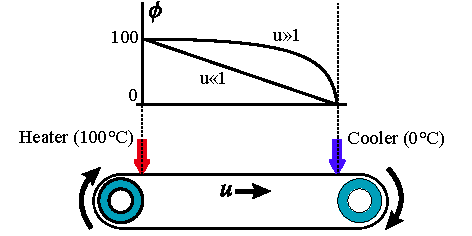
\includegraphics[width=80mm]{images/velt_convayer}
  \caption{Imagine a belt conveyor that send a belt with constant speed $u$. At the upstream location the belt is heated as $\phi=100$ and is cooled at the downatream location $\phi=0$. If the belt runs very slow the temperature of the belt would be linear as the heat diffusion is dominant. If the belt runs fast, the temperature of the belt, advection effect makes the temperature an will be higher than that of linear. }
  \label{fig:lap_domain}
\end{figure}

The figure above is such that two temperatures are given to the upstream side and the downstream side of the belt conveyor moving at a constant speed $u$. The temperature distribution while these two temperatures are given is considered to follow the steady advection diffusion equation.


\subsubsection{General Solution of One-dimensional Steady Advection-Diffusion Equation}
When the above equation is made one-dimensional, the one-dimensional advection diffusion equation is as follows

\begin{equation}
u\frac{\partial \phi}{\partial x}=\nu\frac{\partial^2 \phi}{\partial x^2}
\end{equation}

When the length is $L$ and the values ​​at both ends are fixed, the solution is multiplied as follows.

\begin{equation}
\phi=a e^{\frac{u}{\nu}x}+b
\end{equation}

However, the variable $a,b$ is chosen to satisfy the boundary condition.
Here, if you convert $x$ to a dimensionless length $t$ like $x \rightarrow Lt$
The solution is finally applied as follows.

\begin{equation}
\phi=a e^{\frac{uL}{\nu}t}+b=a e^{Ret}+b
\end{equation}

However, $Re=\frac{uL}{\nu}$ is Reynolds number. (It seems that it is correct to take the absolute value of u but it was kept as it was for the sake of simplicity here.) Since the Reynolds number is on the shoulder of the exponential function, as the Reynolds number gets larger, the value sharply increases It turns out that it changes.

\subsubsection{Changes in solution state due to advection velocity}
Assuming that the value at the boundary is $\phi_0,\phi_1$, the solution is multiplied as follows.

\begin{equation}
\phi=(\phi_1-\phi_0)\frac{e^{Ret}-1}{e^{Re}-1}+\phi_0
\end{equation}

\begin{itemize}
\item In case of $Re\simeq0$ Taylor expansion of $e^{Ret}$, it is $e^{Ret}\simeq 1+Ret$, so it becomes $\phi=(\phi_1-\phi_0)t+\phi_0$. That is, the solution is linear.
\item In the case of $Re>>1$, it becomes $\phi=\phi_0 \quad ( \quad for \quad 0 \le t < 1  \quad ),\qquad\qquad \phi=\phi_1 \quad ( \quad for \quad t=1 \quad ) $.
\item In the case of $Re<<-1$, it becomes $\phi=\phi_0 \quad ( \quad for \quad t=0  \quad ),\qquad\qquad\phi=\phi_1 \quad ( \quad for \quad 0< t\le1 \quad ) $.
\end{itemize}

When $\phi_0=0,\phi_1=1$, these are shown in the figure as follows




\begin{figure}[htbp!]
  \centering
  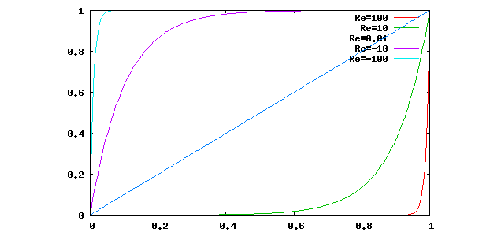
\includegraphics[width=85mm]{images/advec_1d_reynolds}
  \caption{The solutions of one-dimensional stationaly advection equation for various Raynolds numbers}
  \label{fig:lap_domain}
\end{figure}

The command of gnuplot that displays this is as follows

\begin{lstlisting}[caption = gnuplot, label = elem_mat, float, floatplacement = H]
set sample 100
set xrange [0: 1]
title = 'Re = 100', (exp (10 * x) -1) / (exp (10) -1) title 'Re = Ten',}
(exp (0.01 * x) -1) / (exp (0.01) -1) title 'Re = 0.01',}
(exp (-100 * x) -1) / (exp (-100) -1) title 'Re = - 10' title 'Re = -100'}
\end{lstlisting}


\subsection{Upwind Techinique in Finite Difference Method}

It was found that the solution of the advection diffusion equation is basically an exponential function. 
%
When numerical calculation is performed, there are various calculation methods to calculate the first derivative and the second derivative of the solution. 
%
Since it is the accuracy up to the second order in the central difference often used in calculating the first derivative, it can not cope with such an exponential solution. 
%
there, Discretization using upwind difference is often used in the advection term.


\begin{tcolorbox}[title=First order upwind difference method]
\begin{equation}
u\frac{\partial\phi}{\partial x}
=
\left\{\begin{array}{ll}
u\frac{\phi_i-\phi_{i-1}}{h} &  (u>0)\\
u\frac{\phi_{i+1}-\phi_i}{h} & (u<0)
\end{array}\right.
\end{equation}
\end{tcolorbox}

First order upwind difference means \ emph {gradient at the point $x_i$ at the point upstream by 1 / 2h from the point $x_i$ you want to calculate the gradient}.


\subsubsection{Central differential instability and intuitive reason why upwind difference is stable}
The steady advection diffusion equation shows that the gradient of the solution increases as going downwind.
The figure below shows $u>0$, the state of the solution when the wind is blowing from left to right.
%
\begin{figure}[htbp!]
  \centering
  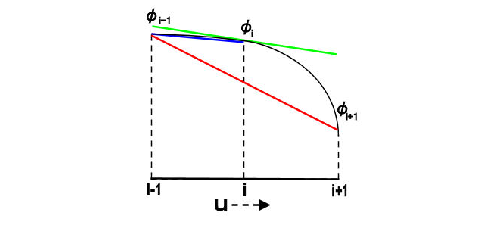
\includegraphics[width=85mm]{images/upwind_central_advec}
  \caption{comparison between central and upwind differential}
  \label{fig:lap_domain}
\end{figure}

The slope of the red line represents the central difference at point $i$, the slope of the blue line represents the upwind difference at point i, the gradient of the green line represents the actual slope at point i
As can be seen from the above figure, we can see that the magnitude of the gradient is evaluated in \emph{the upwind difference method is smaller than it actually is, the central difference is larger than the actual} the gradient magnitude is evaluated.
%
\begin {itemize}
\item When Reynolds number is small, $\phi$ is a straight line, so the central difference and the upwind difference are equal to the actual gradient.
\item If Reynolds number is very large, it becomes $\left.\frac{d \phi}{d x}\right |_i=\frac{\phi_i-\phi_{i-1}}{h}=0$ and the upwind difference coincides with the actual solution. However, it takes a large value deviating in the vicinity of the fixed boundary condition of leeward. Since the term of the second differentiation has to be balanced with this, the convex or concave portion greatly propagates in this part and it propagates to the windward and the solution vibrates near the fixed boundary of leeward.
\end {itemize}



\subsubsection{windward difference method and numerical viscosity}
Using the central difference in the above equation

\begin{equation}
u\frac{\partial\phi}{\partial x} = u\frac{\phi_{i+1}-\phi_{i-1}}{2h} - \frac{|u|h}{2} \frac{\phi_{i+1}-2\phi_i+\phi_{i-1}}{h^2}
\end{equation}

. The second term on the right side of the above equation uses the upwind difference
Therefore, since it is an artificially introduced diffusion term, it is called Artificial Diffusion or Numerical Viscosity. Also, the coefficient of artificial diffusion is called artificial diffusion coefficient.
As shown above, the artificial diffusion coefficient $\nu_{\infty}$ by the upwind difference method is given as follows

\begin{tcolorbox}[title=artificial diffusion coefficient by upwind difference method]
\begin{eqnarray}
\nu^{\infty} = \frac{|u|h}{2}
\end{eqnarray}
\end{tcolorbox}

Using these, the advection diffusion equation introducing artificial viscosity is
By using the central difference, we can write

\begin{equation}
u\frac{\phi^{i+1}-\phi^{i-1}}{2h} - \frac{|u|h}{2}\frac{\phi^{i-1}-2\phi^i+\phi^{i+1}}{h^2} = \nu\frac{\phi^{i-1}-2\phi^i+\phi^{i+1}}{h^2}
\end{equation}


\begin{equation}
u\frac{\phi^{i+1}-\phi^{i-1}}{2h} = (\nu+\nu^{\infty})\frac{\phi^{i-1}-2\phi^i+\phi^{i+1}}{h^2}
\end{equation}

In this case, the upwind difference can be expressed by the original advection diffusion equation

\begin{equation}
u\frac{\partial\phi}{\partial x} = (\nu+\nu^{\infty})\frac{\partial^2\phi}{\partial x^2}
\end{equation}

It is equal to what you rewritten the central difference.



\subsection{Optimization of Artificial Viscosity}

When the influence of the advection term is large
It is known that the above equation coincides exactly with an exact solution
When the influence of advection is small, compared with the actual solution
It is known that numerical solutions are lost.
Therefore, by changing the influence of artificial viscosity according to the influence of advection,
It is possible to make the numerical solution coincide with the exact solution.
Specifically, the artificial viscosity $\nu_{opt}$ should be determined as follows

\begin{equation}
\nu_{opt} = \nu_{\infty} L(\lambda), \qquad \lambda=\frac{\nu_{\infty}}{\nu_{opt}} = \frac{1}{2}\frac{|u|h}{\nu}=\frac{1}{2}Re_c
\end{equation}

Where $Re_c$ is the Cell Reynolds number,

\begin{equation}
L(x) = coth(x)-\frac{1}{x}
\end{equation}

Is a Langevin function.
With $\lambda \rightarrow {\infty}$
Since it is $L(\lambda)=1$, at this time
Become $\nu_{opt}=\nu_{\infty}$.
That is, for a major problem of the advection term
The solution of the first order upwind difference method coincides with the exact solution.
Also, because $\lambda=0$ is $L(0)=0$
If the influence of the advection term is small, the artificial viscosity value is also
It turns out that it becomes small. However, even if
Even if the influence is small, the solution with artificial viscosity added
It is necessary to be careful that it becomes close to an exact solution.
From the above,

\begin{equation}
u\frac{\partial\phi}{\partial x} = (\nu+\nu_{opt})\frac{\partial^2\phi}{\partial x^2}
\end{equation}

Can be discretized with the central difference to obtain an exact solution.





\subsection{application of upwind difference to finite element method}

\subsubsection{Bubnov-Galerkin Method and Central Difference Method}

On the one-dimensional advective diffusion problem, the Bubnov-Galerkin method
It shows that the Finite Element Method and the difference method based on the central difference are equal.
Bubnov-Galerkin method means that the shape function and the weighting function of the interpolation function are equal.
Differential equation

\begin{equation}
u\frac{\partial\phi}{\partial x} = \nu \frac{\partial^2 \phi}{\partial x^2}
\end{equation}


\begin{equation}
{\int^1_0}{\delta\phi}u\frac{\partial\phi}{\partial x}dx = {\int^1_0}{\delta\phi}\nu \frac{\partial^2 \phi}{\partial x^2}dx
\end{equation}


\begin{equation}
{\int^1_0}u{\delta\phi}\frac{\partial\phi}{\partial x}dx = -{\int^1_0}\nu\frac{\partial\delta\phi}{\partial x}\frac{\partial\phi}{\partial x}dx
\end{equation}

By the Bubnov-Galerkin method, a function whose shape function and weight function are equal to each other
It is assumed to be expressed by $N$. In other words,
$\phi = {N^i}{\phi^i}$,

\begin{equation}
\delta\phi = {N^j}{\delta\phi^j}
\end{equation}

Assume that interpolation is performed as shown in Fig. Substituting the above equation into the above equation

\begin{equation}
{\int^1_0}u{N^i\delta\phi^i}\frac{\partial N^j\phi^j}{\partial x}dx = -{\int^1_0}\nu\frac{\partial N^i\delta\phi^i}{\partial x}\frac{\partial N^j\phi^j}{\partial x}dx
\end{equation}

Deleting the weight value $\delta\phi_i$ at node i from both sides

\begin{equation}
{\int^1_0}u{N^i}\frac{\partial N^j\phi^j}{\partial x}dx = -{\int^1_0}\nu\frac{\partial N^i}{\partial x}\frac{\partial N^j\phi^j}{\partial x}dx
\end{equation}

The weight function $N^i$ has a nonzero value
It is in the range of $x=[x_i-h,x_i+h]$.
In this range, the shape function $N^j$ has a nonzero value
It is only when it is $j=i-1,i,i+1$. Therefore, the weight function $N^i$
The following equation holds.

\begin{eqnarray}
u{\int^{x_i+h}_{x_i-h}}  {N^i}\frac{\partial N^{i-1}\phi^{i-1}}{\partial x} + {N^i}\frac{\partial N^i\phi^i}{\partial x} + {N^i}\frac{\partial N^{i+1}\phi^{i+1}}{\partial x}dx\\ = -\nu{\int^{x_i+h}_{x_i-h}}  \frac{\partial N^i}{\partial x}\frac{\partial N^{i-1}\phi^{i-1}}{\partial x} + \frac{\partial N^i}{\partial x}\frac{\partial N^i\phi^i}{\partial x}dx + \frac{\partial N^i}{\partial x}\frac{\partial N^{i+1}\phi^{i+1}}{\partial x}dx
\end{eqnarray}

When this integration is executed, the following expression is obtained.

\begin{equation}
u\frac{\phi^{i+1}-\phi^{i-1}}{2h} = \nu\frac{\phi^{i-1}-2\phi^i+\phi^{i+1}}{h^2}
\end{equation}

It discretized this problem using the central difference method Equation.
%
Therefore Bubnov-Galerkin method and the central difference method is the same in one dimensional steady advection diffusion problem.






\subsubsection{Adaptation of Upwind Difference to Finite Element Method}1

Appropriate artificial viscosity for central difference $\nu_{opt}$
To introduce a numerical solution to an exact solution
I found out that I can do it.
Therefore, even in the case of the finite element method, the artificial viscosity $\nu_{opt}$
It is necessary to make a numerical solution an exact solution by adding
Can be considered.
The weak form with artificial viscosity added is as follows

\begin{equation}
u\frac{\partial\phi}{\partial x} = (\nu+\nu_{opt})\frac{\partial^2 \phi}{\partial x^2}
\end{equation}

With reference to the above equation, the discretization of this equation by the finite element method

\begin{equation}
{\int^1_0}{N^i}u\frac{\partial N^j\phi^j}{\partial x}dx = -{\int^1_0}(\nu+\nu_{opt}) \frac{\partial N^i}{\partial x}\frac{\partial N^j\phi^j}{\partial x}dx
\end{equation}

.
When this equation is modified and the term of artificial viscosity is moved to the advection term on the left side

\begin{equation}
 {\int^1_0}(N^i+\frac{\nu_{opt}}{u}\frac{\partial N^i}{\partial x})u \frac{\partial N^j\phi^j}{\partial x}dx = -{\int^1_0}\nu\frac{\partial N^i}{\partial x}\frac{\partial N^j\phi^j}{\partial x}dx
\end{equation}

. The meaning of this expression is that the left side of the above equation
Weight function for weak form advection term

\begin{equation}
 N^i \quad \rightarrow \quad \bar{N}^i\equiv N^i+\frac{\nu_{opt}}{u}\frac{\partial N^i}{\partial x}
\end{equation}

It is equivalent to deforming as shown in Fig.
This shape function $\bar{N}^i$ has the original shape function $N^i$
, The weight on the windward side is larger and the weight on the leeward side is smaller
It shows that it has the same effect as the upwind difference.



\section{Stabilization of Multi-dimensional Advection-Diffustion Problem}
%
The steady advection diffusion equation in multidimension is multiplied as follows.

\begin{equation}
 {\bi{u}}\cdot(\nabla_x\phi) = \nabla_x \cdot (\nu\nabla_x\phi)
\end{equation}

For the steady one-dimensional advection diffusion equation, the numerical viscosity coefficient is added to the viscosity term
Add, discretize by the Bubnov-Galerkin method
We were able to obtain the solution with high accuracy by doing.
However, by adding the numerical viscosity coefficient as it is to the viscous term of the above equation

\begin{equation}
{\bi{u}}\cdot(\nabla_x\phi) = \nabla_x \cdot \{(\nu+\nu_{opt})\nabla_x\phi\}
\end{equation}

Discretized by the Bubnov-Galerkin method
It is known to give unnatural and unrealistic solutions.
%
The original idea of ​​the upwind difference is that of the advection term in the windward direction Move the calculation point to add numerical diffusion in the streamline direction It was.
%
However, the above formula merely increases the viscosity,Not only does it add numerical diffusion in the streamline direction, Since numerical diffusion is also applied to the direction perpendicular to the streamline direction
It is a problem because the viscosity becomes larger than it actually is.
Therefore, consider adding a numerical diffusion term only in the streamline direction.
%
As preparation for that Consider the spatial differentiation operator of streamline direction $\bi{e}_s$ as follows.
%
\begin{equation}
\frac{\partial}{\partial x_s} = {\bi{e}_s} \cdot \nabla_x \otimes = \frac{\bi{v}}{|{\bi{v}}|} \cdot \nabla_x \otimes = \frac{v_i}{|{\bi{v}}|} \frac{\partial}{\partial x_i}
\end{equation}

Using this operator, for example,

\begin{equation}
\frac{\partial \mathcal{A}}{\partial x_s}
\end{equation}

Is the physical quantity along the streamline direction $\bi{e}_s$  Of the change per unit length, It is a gradient in the streamline direction.
%
Multidimensional steady advection diffusion equation expressed by the above equation.
%
The equation with the artificial viscosity coefficient in the streamline direction added to it can be written as

\begin{equation}
 {\bi{u}}\cdot(\nabla_x\phi) = \nu \nabla^2\phi + \frac{\partial}{\partial x_s} \left( \nu_{opt} \frac{\partial\phi}{\partial x_s}\right)
\end{equation}


\begin{equation}
{\bi{u}}\cdot(\nabla_x\phi) = \nu \nabla^2 \phi + {\bi{e}_s} \cdot \left[ \nabla_x \{\nu_{opt}{\bi{e}_s}\cdot (\nabla_x\phi)\}\right]
\end{equation}

Weak formalization of the above equation

\begin{equation}
\int_v {\delta\phi}{\bi{u}}\cdot(\nabla_x\phi) dv = -\int_v \nu \nabla_x{\delta\phi} \cdot \nabla_x\phi + {\delta\phi}{\bi{e}_s} \cdot \left[ \nabla_x\{\nu_{opt}{\bi{e}_s}\cdot(\nabla_x\phi)\}\right] dv
\end{equation}

Modify the third term on the right side.

\begin{eqnarray}
&&\int_v \delta\phi{\bi{e}_s} \cdot \left[ \nabla_x\{\nu_{opt}{\bi{e}_s}\cdot(\nabla_x\phi)\} \right] dv\\
&=& \int_v {\bi{e}_s} \cdot \left[ \nabla_x \{ \nu_{opt}{\delta\phi}{\bi{e}_s}\cdot(\nabla_x\phi)\} \right] - \{{\bi{e}_s}\cdot(\nabla_x{\delta\phi})\} \{\nu_{opt}{\bi{e}_s}\cdot(\nabla_x\phi)\} dv\\
&=& \int_v \nabla_x \cdot \left[ \{{\delta\phi}\nu_{opt}{\bi{e}_s}\cdot(\nabla_x\phi)\} {\bi{e}_s}\right] - \underbrace{\left\{\nabla_x \cdot {\bi{e}_s}\right\}}_{=0} \{{\delta\phi}\nu_{opt}{\bi{e}_s}\cdot(\nabla_x\phi)\} - \{{\bi{e}_s}\cdot(\nabla_x{\delta\phi})\} \{\nu_{opt}{\bi{e}_s}\cdot(\nabla_x\phi)\} dv
\end{eqnarray}

Apply Gauss' divergence theorem to the first term.
%
Also, if the streamline direction $\bi{e}_s$ is constant, The second term is $0$. 
%
Thus, the above equation

\begin{eqnarray}
&&\int_s{\bi{n}}\cdot\underbrace{\left[ \{{\delta\phi}\nu_{opt}{\bi{e}_s}\cdot(\nabla_x\phi)\}{\bi{e}_s} \right]}_{=0}ds 	- \int_v\{{\bi{e}_s}\cdot(\nabla_x{\delta\phi})\}\{{\nu_{opt}}{\bi{e}_s}\cdot(\nabla_x\phi)\} dv\\
&=& -\int_v\{{\bi{e}_s}\cdot(\nabla_x{\delta\phi})\} \{{\nu_{opt}}{\bi{e}_s}\cdot(\nabla_x\phi)\} dv\\
&=& -\int_v\{\frac{\bi{v}}{|\bi{v}|}\cdot(\nabla_x{\delta\phi})\} \{{\nu_{opt}}\frac{\bi{v}}{|\bi{v}|}\cdot(\nabla_x\phi)\} dv\\
&=& -\int_v\{\frac{\nu_{opt}}{|\bi{v}|^2}{\bi{v}}\cdot(\nabla_x{\delta\phi})\} \{{\bi{v}}\cdot(\nabla_x\phi)\} dv
\end{eqnarray}

It is transformed into the equation. Substituting this into the above equation

\begin{equation}
\int_v \left\{{\delta\phi}+\frac{\nu_{opt}}{|\bi{v}|^2}{\bi{v}}\cdot(\nabla_x{\delta\phi})\right\}\left\{{\bi{v}}\cdot(\nabla_x\phi)\right\} dv = -\int_v\nu \nabla{\delta\phi} \cdot \nabla{\phi}
\end{equation}

This is because the weight function $\delta\phi$ of the advection term is replaced with $\delta\bar{\phi}$
It is equivalent to changing.

\begin{equation}
 \delta\phi \quad \rightarrow \quad \delta\bar{\phi} = {\delta\phi}+\tau{\bi{v}}\cdot(\nabla_x{\delta\phi})
\end{equation}

However, $\tau$ is a stabilization parameter defined below.
{\ bf Stabilization parameter}
, $\tau = \frac{\nu_{opt}}{|\bi{v}|^2}$
The numerical diffusion added here will be examined in detail.
When transforming the term of numerical diffusion,

\begin{eqnarray}
{\bi{e}_s} \cdot \left\{ \nabla( \nu_{opt} {\bi{e}_s} \cdot {\nabla\phi} ) \right\} \\ = \nabla\cdot \left\{{\bi{e}_s}(\nu_{opt}{\bi{e}_s}\cdot{\nabla\phi})\right\} - \underbrace{(\nabla\cdot{\bi{e}_s})}_{=0} (\nu_{opt}{\bi{e}_s}\cdot{\nabla\phi})\\									=\nabla\cdot(\underbrace{(\nu_{opt}{\bi{e}_s}\otimes{\bi{e}_s})}_{Tensor \quad Viscosity}\cdot{\nabla\phi})
\end{eqnarray}

Changes in the direction of streamlines were negligible. here

\begin{equation}
\nu_{opt}{\bi{e}_s}\otimes{\bi{e}_s} = \nu_{opt}\frac{\bi{v}}{|\bi{v}|}\otimes\frac{\bi{v}}{|{\bi{v}}|} = \frac{\nu_{opt}}{|\bi{v}|^2}{\bi{v}}\otimes{\bi{v}} = \tau{\bi{v}}\otimes{\bi{v}}
\end{equation}

Is called tensor viscosity. It has anisotropy such that there exists a value that becomes viscous only in the direction of the streamline.
\subsection{Discretization of Finite Element Method of Multidimensional Advective Diffusion Problem}
\subsection{stabilization parameter of multidimensional problem}
The stabilization parameters are expressed as follows.

\begin{equation}
\tau = \frac{\nu_{opt}}{||\bi{v}||^2}
\end{equation}

$\nu_{opt}$ makes the solution at the node consistent with the exact solution in one dimension as follows.
$\nu_{opt} = \frac{||\bi{v}||h}{2}(\coth(\lambda)-\frac{1}{\lambda})$,

\begin{equation}
\lambda=\frac{1}{2}\frac{||\bi{v}||h}{\nu}
\end{equation}

Where $h$ is the mesh size. In the case of one dimension, the mesh size is equal to the length of the line element, so there is no particular problem, but in the case of two dimensional three dimensions the mesh size is not easily determined. For two- and three-dimensional elements $h$ must be representative of the length of the element in the direction of flow velocity.
In the paper of 1991 (Tezduyar, TE: "Stabilized finite element formulation for incompressible flow computations", Advance in Applied Mechanics, Vol. 28, pp. 1-44 (1991))) The mesh size in the direction is determined.

\begin{equation}
h = 2 \left( \sum_{a=1}^{n} \left|\bi{s} \cdot \nabla_x \bi{N}_a \right|\right)^{-1}
\end{equation}

Where $n$ is the number of interpolation functions of the element. Also, $\bi{s}$ is a direction vector normalized to a length of 1 by flow velocity vector $\bi{v}$.
In addition, the following approximation is used in this paper.

\begin{eqnarray}
\coth(\lambda)-\frac{1}{\lambda}\simeq z(\lambda)
=\left\{\quad\begin{array}{l}
\frac{1}{3}\lambda\\
1
\end{array}
\qquad\qquad
\begin{array}{l}
(\quad 0\le\lambda\le3 \quad )\\
(\quad 3 < \lambda \quad )
\end{array}\right.
\end{eqnarray}

The function before the approximation function z is approximated is shown in the following graph


%file: zapp_lang.png


\section{sample program}

\subsection{Problem setting}
The next sample program is the following in the rectangular area of ​​size 1 x 1
It is a problem to solve the advection diffusion equation.

\begin{equation}
\bi{u}\cdot\nabla\phi-0.001{\nabla}^2\phi=0 \qquad ( \quad in \quad \Omega = \{x,y:-0.5<x,y<0.5 \} \quad )
\end{equation}


\begin{eqnarray}
\bi{u}=\left(
\begin{array}{l}
x\\
-y
\end{array}\right)
\end{eqnarray}


\begin{eqnarray}
\left\{\begin{array}{l}
\phi=0 \qquad ( \quad on \quad \partial\Omega \quad ) \\
\phi=(\sin2\pi x)^5 \qquad ( \quad on \quad \{x,y:0.0<x<0.5,y=0.0 \} \quad)
\end{array}\right.
\end{eqnarray}

file: doughnuts.jpg
There is a notch passing through the origin in the rectangular area, and there is a fixed boundary condition in it.
The flow velocity is assumed to flow counterclockwise so as to draw a circle around the origin.
The discretization of the problem uses the stabilized finite element method.


\subsection{download}
| ~ DOWNLOAD | [[GMRes.zip> file: GMRes.zip]] |
 OS: Windows XP, Windows 2000
 Development environment: VC ++ 2005
 Language: C ++
 
 

\subsection{Show Results}
When we run the program we call 'solution.dat'
A result file is generated.
'solution.dat' has data format for gnuplot
Introduction of windows version of gnuplot, the following page is detailed
: Introductory gnuplot introduction | http: //auemath.aichi-edu.ac.jp/~khotta/ghost/gnuplot.html
: Physical key tail (initial setting of Windows version of Gnuplot) | http: // hooktail.org/computer/index.php? Windows% C8% C7Gnuplot% A4% CE% BD% E 9% B 4% FC% C 0% DF % C 4% EA


\subsubsection{Show Surface with Height in Height}

After starting gnuplot, move to the directory of 'solution.dat' which executed the program and hit the following command and the result is displayed.
 gnuplot> set style data line
 gnuplot> splot 'solution.dat'
%file: doughnuts_hight.png

\subsubsection{Display Contour Lines}
Also, when you type the following command, gnuplot displays contour lines like the one below.

 gnuplot> set nosurface
 gnuplot> set contour base
 gnuplot> set view 180,90
 gnuplot> splot 'solution.dat'
 
 
%file: doughnuts_contour.png



\end{document}
